
{\bf \Huge Research Plan} \\[0.5cm]

  My research is divided into two phases, a research project in the fall and master thesis in the following spring. This research plan will cover both phases.

  \section*{Purpose}

  \begin{comment}
    Describe the reason for doing the research, the topic of interest, why it is important or useful to study this, the specific research question(s) asked and the objectives set. Research without a purpose is unlikely to be good research. (Oates 2005)
    Write in this section about the following:
    ·       What is the problem? Whose problem is it? Refer to 2-3 good scientific references that confirm for the reader that this is actually a relevant problem.
    ·       What is done earlier to address this problem? Give 4-5 good references that illustrate the different approaches taken by other researchers to solve this problem. (you might also consider to do an in-depth literature review as part of your autumn project).
    ·       What is wrong with earlier research? Did they not manage to solve the problem? Why? Why is your approach going to be better? What new knowledge do you plan to add?
    ·       Summarize with a list of clearly defined research questions. One main question and 2-3 sub-questions related to the main question. Note that the sub-questions should contribute to answer the main question.
  \end{comment}

  \begin{comment}
    In todays society, people tends to spend a lot of time on their mobile devices. Mobile devices are not just a communication tool, but also an important tool for everyday tasks like doing our work, reading mail, pay our bills, and keeping up with our social life. Our whole life is contained in one device. When such a small device is so important it makes it vulnerable in terms of security.

    Passwords are human-chosen secrets that are connected to you as a person. When the password is created you might create a password that is an association to something you know or recognize; passwords are more than just words and numbers. Because of the shortcomings of text-based passwords \cite{UnixPasswords}, there is an increased interest in graphical passwords. The interest in graphical passwords started with the assumption that pictures are easier to remember and more secure than words and numbers \cite{DeAngeli}. Google's Android platform released the functionality for the Android Unlock Pattern in 2008, that is a security mechanism for locking Android smartphones. Since its release, there have been a lot of discussion regarding its security, but little scientific research on the Android Unlock Pattern. The problem is not just the theoretical password space, but the password space in practice. 

    The motivation for this thesis started by observing the shortcomings of graphical passwords. Password reuse is one of the known password habits among users because of the human limitation in remembering text-based passwords. Some users also make simple or semantic passwords that are easier to remember, making their passwords vulnerable to attacks. Graphical passwords look like a promising alternative to text-based passwords, as it aids users in remembering and create more complex passwords, offering increased usability and higher security. As mobile devices play an important role in our everyday life, this makes it an interesting target device. Security on mobile devices have changed during the past years. Historically, locking mechanisms were a solution solely to prevent accidental use, while current mobile phones require protection in order to secure the potentially vast amount of private data that we keep on them.

    In 2013 a research group conducted the first large-scale user study on the Android Unlock Patterns \cite{Uellenbeck}. The outcome of the research was an analysis of 2900 collected Android Unlock Patterns. They found a lot of bias in the pattern making process claiming that the scheme is less secure than its theoretical password space. 

    My research aims to take the analysis of people's choice in Android Unlock Patterns a step further by including the human properties that may impact the user choice in graphical passwords. The study adds to the body of knowledge by testing the hypothesis that human properties affects user's choice of graphical passwords. It is also desired to look into further improvements of the scheme. 

    {\bf $RQ1$: What is the status of current research on graphical passwords?}

    {\bf $RQ2$: What human properties may affect our choice of graphical passwords on mobile devices?}

    {\bf $RQ3$: How is users choice of patterns based on human properties affecting the security of the Android Unlock Pattern?}

    {\bf $RQ3.1$: If any security risks is observed, how could the Android Unlock Pattern scheme be improved in order to reduce the security risks?} 

    Mitt:

    As online stores are easy to access and users are not always sure what they want, it could be useful to help guide users to the products that are interesting for them. As this is already done in a lot of different ways, it could be useful to also look for better ways to utilize this in search. Online stores have access to more descriptive information about their products than what free text search can offer. Helping users easier find what they are after could raise revenues for online stores [link til produktet som gjør det.]

  \end{comment}

  \begin{comment}
  There is a lot of work being done with query suggestions [Ikke query suggestion, men søke-fagfeltet], and studies show it is helpful for users as they more quickly get the results they want [link to relevant information]. There is already many search engines utilizing personalized query suggestions such as Google and Facebook. As the web is huge and most users are not good at formulating accurate and precise queries, it has been shown in various research that this has a positive effect.

  Most research on personalized query is regarding free-text search, as this is an area particularly hard area for users [Link]. The way user thinks and the way the query engine process data does not always match to well.

  There is also a lot of work being done with personalizing stores for the users. Amazon with does this with similar products, app stores show recommended apps as well as showing you what similar users and friends have bought. Still the search engine being used in most online stores are lacking behind when it comes to personalization for users. Users usually have to first type in a search, then they will get redirected to where they want. This research will investigate methods to instantly recommend desired apps for users based on personal information about them. I will investigate different methods to perform these suggestion. The focus will be on query suggestion, query completion and recommending apps more based on user preferences than directly the search term. [Må finne bedre navn for det siste]

  A lot of the work being done on personalized query suggestions are in a free-text search domain, like Google, even though there are a lot of examples of other search engines utilizing the same techniques.

  \end{comment}

  Search is an important part of our web experience today. There is a lot information on the web, and search is a good tool to find the information [link?]. The problem is that most people present short, unprecise and ambiguous queries to search engines, which leads to bad results being presented to the users[link]. Because of this there is a lot of work in the field of helping the users find the information they want. Query suggestion and query completions are such methods, which helps users formulate good queries. These suggestions benefit from being personalized to the given user [link], as different users can look for different things even thought they type the same query [apple example]. There are many companies using personalized search engines today, such as Google, Facebook and Amazon [Ref?].

  Many web stores today are personalized for the users. They utilize methods such as suggesting products, recommending products and product placement based on preferences, friends or similar users. All these methods are used in app stores such as Google Play. Still with all this work on personalization most of their search engines are only personalized to a limited degree [link]. This project will work with analyzing different methods for personalizing query engines for app stores, and see if search engines could perform better if they are personalized. If users are able to find apps they want to download quicker, either apps they are searching for or apps they were unaware of beforehand, this should be beneficial for app stores and their users. Different methods that will be suggested is personalized query suggestion and query completion and ranking suggestions based on users preferences. The query suggestion will both have a section with more focus on the query typed in, and a section more focused on the users preferences. Even though these are methods that could be tested in web stores in general this project focus on app stores.

  There are a lot of research that could be done in this field, the questions I will focus on are
  \newline

  {\bf $RQ1$: What is the status of current personalized search engines in online stores today?}

  {\bf $RQ2$: How can we improve the methods of personalized search in app stores?}

  {\bf $RQ3$: Does instant personalized search engines outperform search engines used in app stores today?}

  
  \section*{Contribution} %product

  \begin{comment}
  The main product of this research is to test a hypothesis in mobile security. The hypothesis states that there is a connection between users' choice in graphical passwords based on human properties like physical conditions and demographics. Towards reaching this goal, there are other sub-products of the research process. The literature review and the research design is two sub-products delivered in the project thesis. In my master thesis, a data collection and quantitative data analysis is conducted. The data itself is a valuable product, and alongside with the analysis, it can provide answers to the hypothesis.

  Research on passwords is not easy to conduct because of the nature of passwords. Passwords should not be shared. Research on text-based passwords is often based on leaked password on the web. When analyzing Android Unlock Patterns, there is no such data source available. This research design can provide insight into a new way of solving the problem of collecting user chosen passwords on mobile devices. The research design provides a detailed description of the strategy chosen to collect Android Unlock Patterns from users through a questionnaire over the Internet. This can provide knowledge for future research on graphical passwords on mobile devices. 
  \end{comment}

  The main product of this project is to research and evaluate different methods for instant personalized search. The hypothesis states that instant personalizing search for users will make it easier to find apps they want, either apps they are searching for or apps they like and previous was unaware of. Research points to that personalized query suggestion and recommendation is efficient in free-text search, such as Google's search engine, but this paper will research the effects in online app stores with more structured data. The prototype will act as a research platform and test for this research, but can also be used and modified by others for further research.

  The result of this research will also evaluate on whether instant personalized search or outperform other methods which are more used today, such as suggestions based on most popular or highest ranked products [link]. There are many different online stores implementing personalization of different parts of their site [link], including their search engines. This research will evaluate methods used by these search engines and try to develop personalized search further.
  
  \section*{Research} %process

  \begin{comment}
  \begin{wrapfigure}{l}{0.53\textwidth}
     \vspace{-20pt}
     \begin{center}
        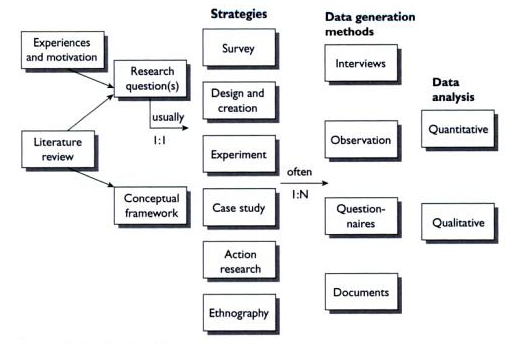
\includegraphics[scale=0.13]{ResearchProcess.png}
     \end{center}
     \vspace{-5pt}
     \caption{Research Process \cite{empiriske}}
   \end{wrapfigure}

  This research spurred by the experience and motivation that graphical passwords are an interesting form of authentication, supporting users to remember more complex passwords that should provide better security. To find the research questions, I started with a literature review, providing a conceptual framework for the thesis. From the literature review, I found that there is a lack of research on human choices of graphical passwords based on human properties. Beside the literature review, the research project also includes a research design for my master thesis. In order to find out if there is possible to see a pattern between users choice in passwords and human properties, a survey is planned along with a questionnaire for the data collection. The research requires a large sample of data for finding patterns in users' choice of Android Unlock Patterns, as well as diversity in the data in terms of demographics. With today's technology it is possible to distribute the questionnaire over the Internet. A questionnaire also provides a standardized format of the data that can be helpful for the analysis. The selected research strategy and data generation method will provide quantitative data for the analysis.
  \end{comment}

  \begin{wrapfigure}{l}{0.53\textwidth}
    \vspace{-20pt}
    \begin{center}
      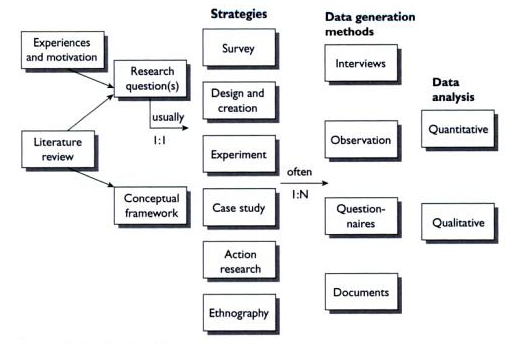
\includegraphics[scale=0.5]{ResearchProcess.png}
    \end{center}
    \vspace{-5pt}
    \caption{Research Process \cite{empiriske}}
  \end{wrapfigure}

  The area of big data and search is a fast growing and interesting area for research. I chose this project as one of the research questions from my supervisor, and it felt like at natural choice as this is, in my opinion, an interesting research field. There is a lot of work being done with big data, personalization and search, and tying it all together could prove interesting and useful.

  I started with a literature review and conceptual framework for the thesis. With focus on how existing online store does search and personalization for users, and see if there are similar or existing solutions to the search engine that will be tested in this research.

  Keywords for further writing:

  Write more about the process after this.

  Will do surveys for for existing data, design and create a prototype that I will use for experimenting and testing on users.

  I will need a crawler to find information about apps that I can use, and also some form of text summarizer for generating structured data from apps.

  Then I will perform a test on some users to see if the instant personalized system performs better than a simple ``dumb'' search. This test will also contain a questions for the users in order to get qualitative data.

  I will then do a hybrid of quantitative and qualitative analysis on the data from the tests to evaluate the system.



  \section*{Participants}

  \begin{comment}

  As a researcher, I am included as a participant. My work is to plan and conduct the research. 

  The research is supervised by Lillian Røstad and Per Thorsheim. Lillian is my main supervisor and is contributing with her experience with research in computer science and security. Per has the role as my co-supervisor and is an external participant outside of the academic field. He is contributing in this research because of his personal interest in passwords and security, as well as providing a network of contacts within the field of information security. Both have the right to the results form this research.

  In this research, there is not a narrow target population. The aim is to collect data world wide: Everyone with a smartphone is considered a part of the target population. All the volunteered respondents are considered participants in this research. Myself, as a researcher, have no personal contact with the respondents, but need to carefully handle the information from the respondents according to a legal and ethical perspective. It should not be able to track the information back to the respondents. All the data from the respondents are kept anonymous and will not be used outside of this research. Information concerning legal and ethical aspects of this research should be described in the questionnaire. 

  I also need access to information about apps in a online store. This is for the apps to be authentic and accurate for the tests. These apps will be used by the search engine created to evaluate the system. As of today there is no easy way to get the information needed, so I will have to crawl the stores for all information and structure the data myself.

  \end{comment}

  I am included as a participant as the researcher. My work is to plan and conduct the research. I will also create and evaluate the system used for testing the personalized instant recommendation.

  The supervisor of the research is Heri Ramampiaro who also suggested this topic. He will be contributing with his experience in the field of information retrieval and big data.

  I will also need to test my system on a user group to evaluate my system. Any person familiar with app stores would be relevant for this test. These users can be other students at NTNU that can be kept anonymous. As a researcher I will have no personal contact with the participants and handle information according to all ethical and legal perspectives. The data will not be used anywhere else than this research, and the users have to confirm to providing this information for the research.

  [Fyll in eventuelle mennesker eller andre jeg må ha kontakt med for å kunne forske på dette]

  \section*{Research paradigm} %paradigm
  \begin{comment}
  With a survey as the a chosen research strategy, this research seeks to find patterns that are assumed to exist. This is a way of thinking is closely related to the positivism paradigm. This research is based on empirical testing of a hypothesis, with a desire to confirm or refuse the assumptions made in the hypothesis.
  When conducting the research, my beliefs as a researcher are independent of my research and my research can be stated to be objective. It is conducted with minimal interaction with the participants and the research is based on facts, that is the the quantitative data collected. 
  \end{comment}

  \section*{Final deliverables and dissemination} %presentation

    The presentation of the result from this research will be presented in two deliverable documents, project thesis and master thesis. I will also create a prototype to test my research on, which will also be part of the deliverables. This will be an open source project that can be used in further research.
    
  \begin{comment}
  The presentation presentation of the result from this research will be presented in two deliverable documents, project thesis and master thesis. The research will also be presented at the conference ``Passwords14''\cite{passwords} in December. The presentation will provide insightful feedback from researcher, as well as providing knowledge about the gap in the research on graphical passwords. 
  \end{comment}



  \section*{References}
  \renewcommand{\bibsection}{ }
  \bibliographystyle{plain}
  \bibliography{mybib}







  